%%% File encoding: UTF-8
%%% äöüÄÖÜß  <-- keine deutschen Umlaute hier? UTF-faehigen Editor verwenden!

%%% Magic Comments zum Setzen der korrekten Parameter in kompatiblen IDEs
% !TeX encoding = utf8
% !TeX program = pdflatex 
% !TeX spellcheck = de_DE
% !BIB program = biber

\documentclass[master,german,smartquotes]{hgbthesis}
% Zulässige Optionen in [..]: 
%   Typ der Arbeit: diploma, master (default), bachelor, internship
%   Hauptsprache: german (default), english
%		smartquotes: zur vereinfachten Eingabe von Hochkommas (nur "...")
%%%----------------------------------------------------------

\usepackage{subfig}
\usepackage{makecell}
\RequirePackage[utf8]{inputenc}		% bei der Verw. von lualatex oder xelatex entfernen!

\graphicspath{{images/}}    % Verzeichnis mit Bildern und Grafiken
\logofile{logo}							% Logo-Datei = images/logo.pdf (\logofile{}, wenn kein Logo gewünscht)
\bibliography{references}  	% Biblatex-Literaturdatei (references.bib)

%%%----------------------------------------------------------
% Angaben für die Titelei (Titelseite, Erklärung etc.)
%%%----------------------------------------------------------

%%% Einträge für ALLE Arbeiten: -----------------------------
\title{Anbindung der Google V8 Javascriptengine an ein Multi-Agent-SCADA-System}
\author{Daniel Giritzer BSc.}

%\programtype{Fachhochschul-Bachelorstudiengang}		% select/edit
\programtype{Fachhochschul-Masterstudiengang}

\programname{Embedded-Systems-Design}
\placeofstudy{Hagenberg}
\dateofsubmission{2021}{08}{23}	% {YYYY}{MM}{DD}

\advisor{FH-Prof. Dipl.-Ing (FH) Franz Wiesinger}	% optional

\strictlicense		%%% restrictive license instead of Creative Commons (discouraged!)

%%%----------------------------------------------------------
\begin{document}
%%%----------------------------------------------------------

%%%----------------------------------------------------------
\frontmatter                    % Titelei (röm. Seitenzahlen)
%%%----------------------------------------------------------

\maketitle
\tableofcontents
\setlength{\parindent}{0pt}
%\include{front/vorwort} 				% Vorwort ist optional
\chapter{Kurzfassung}

Aufgrund der Unterschiede zwischen den einzelnen Anlagen der Automatisierungsindustrie und der unterschiedlichen 
kundenspezifischen Projektanforderungen ist die Anlagenintegration von Multi-Agent-SCADA 
(Supervisory Control And Data Acquisition) Systemen oft mit vielen unvorhersehbaren und komplexen Problemen verbunden. 
Um diese Probleme zu lösen, ist ein einfacher Weg zur Entwicklung und Anpassung vor Ort erforderlich. \\

Eine Möglichkeit, dies zu erreichen, besteht darin, dem Systemintegrator eine dynamisch erweiterbare Skriptsprache mit 
Debugging-Funktionen und einer Interaktionsmethode für den Fernzugriff auf das SCADA-System bereitzustellen.
Javascript eignet sich für diesen Zweck, da online und offline Literatur dazu gefunden werden kann. Außerdem gibt es viele 
öffentlich verfügbare Komponenten und Bibliotheken, um die Sprache zu erweitern, und die meisten Interpreter 
verfügen über Debugging-Protokolle, die die Entwicklung vereinfachen. \\

Die folgende Arbeit beschreibt, wie die Google V8 Javascript Engine in das kommerzielle WinCC OA 
(Windows Control Center Open Architecture) Multi-Agent-SCADA System für Windows und Linux als Teil des
Produktes \textit{SiPlant} eingebettet wird. 
Dies geschieht durch die Implementierung eines dedizierten Agenten, der in der Lage ist, Javascript-Code unter Verwendung dieser
von Google entwickelten Engine auszuführen. \\

Der neu entwickelte Agent erweitert die Skriptsprache um einen Satz von benutzerdefinierten Befehlen, die den Zugriff 
auf die Daten des gesamten Systems durch die Verwendung der ereignisbasierten Konzepte von WinCC OA ermöglichen. \\

Abschließend wird der erstellte Agent in der Praxis auf verschiedenen Plattformen und Projekten untersucht.
		
\chapter{Abstract}


\begin{english}
Due to the difference of every plant in the automation industry and the varying customer-specific project requirements, 
plant integration of multi-agent SCADA (Supervisory Control And Data Acquisition) systems often comes along with 
many unforeseen and complex problems. To overcome these problems, a simple way for on-site engineering and
customization is needed. \\

This can be achieved, by providing the system integrator a dynamically extendable and well-documented scripting language 
with advanced debugging capabilities and an interaction method to access the SCADA system remotely. Javascript fits this 
purpose, as there can be literature found online and offline. Also, there are many publicly available components and libraries
to extend the language and most interpreters feature debugging protocols which help to ease the development. \\

The following thesis describes how the Google V8 Javascript Engine is embedded as a part of the \textit{SiPlant} product 
into the commercial WinCC OA (Windows Control Center Open Architecture) Multi-Agent-SCADA System for Windows and Linux. 
This is done by implementing a dedicated agent which is capable of executing Javascript code by utilizing 
the formerly named engine developed by Google. \\

This custom agent extends the scripting language by a set of custom commands which allow accessing the data of the whole 
system by using WinCC OA's event-based concepts. \\

Finally, the created agent is examined in practice on different platforms and projects.
\end{english}

			

%%%----------------------------------------------------------
\mainmatter          % Hauptteil (ab hier arab. Seitenzahlen)
%%%----------------------------------------------------------

\chapter{Einleitung}
\label{cha:Einleitung}

In diesem Kapitel wird die behandelte Problemstellung und Motivation der vorliegenden Arbeit dargestellt und eine Zielsetzung definiert. Außerdem wird auf die Gliederung
dieser Arbeit eingegangen und der Inhalt der einzelnen Kapitel kurz erläutert.

\section{Motivation für den Einsatz von SCADA-Systemen}

Ein grundlegendes Problem bei der Digitalisierung von Fabriken ist, dass Cloudanwendungen, die Anlagen 
steuern und überwachen wollen, und Anlagen, wiederum deren Daten in der Cloud ablegen wollen. 
Um diesen Konflikt zu lösen, werden sogenannte SCADA-Systeme eingesetzt. SCADA ist ein Akronym und steht für Supervisory Control And 
Data Acquisition. Diese Systeme implementieren laut Automatisierungspyramide Ebene zwei und Teile von Ebene drei. 

\begin{figure}[h]
	\centering 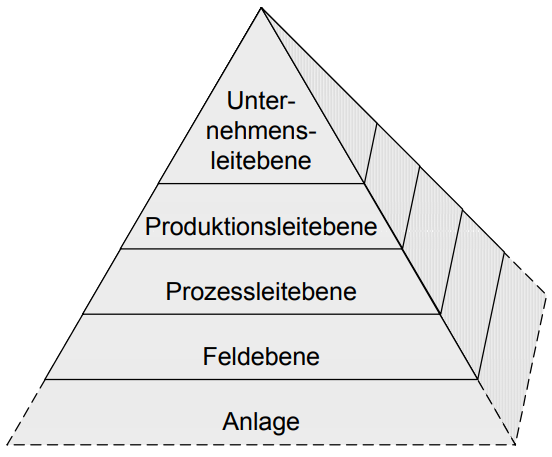
\includegraphics[width=0.58\textwidth]{aut_pyr}
	\caption{Diese Abbildung stellt die verschiedenen Ebenen der industriellen Fertigung mit Hilfe der Automatisierungspyramide dar \cite{automPyr}.
  Cloudanwendungen befinden sich in der Ebene vier, die auch \textit{Unternehmensleitebene} genannt wird.}
	\label{fig:aut_pyr}
\end{figure}

Die in Abbildung \ref{fig:aut_pyr} gezeigten Ebenen können wie folgt zusammengefasst werden \cite{Prozessleittechnik}:
\begin{itemize}
  \item Ebene vier: Die \textit{Unternehmensleitebene} umfasst Produktionsplanung und Bestellabwicklung.
  \item Ebene drei: Stellt die \textit{Produktionsleitebene} dar, in der Produktionsdaten erfasst werden. Außerdem findet hier Qualitäts- und Materialmanagement statt.
  \item Ebene zwei: In der \textit{Prozessleitebene} wird bedient, beobachtet, es werden Daten gesammelt und archiviert.
  \item Ebene eins: Steuert die Anlage über SPSen (Speicherprogrammierbaren Steuerungen), die mit dieser über Bussysteme verbunden sind. Daher wird diese Ebene auch \textit{Steuerungsebene} oder \textit{Feldebene} genannt. Weitere Teilnehmer sind unter anderem Frequenzumrichter und Industrie-PCs.
  \item Ebene null: Als \textit{Anlage} wird die zu steuernde Maschine und die dazugehörige Sensorik bezeichnet. \\
\end{itemize}

Unter SCADA versteht man das Überwachen und Steuern technischer Prozesse durch Computersysteme \cite{whatIsScada}.
Diese Systeme helfen bei der Überwachung von Anlagen und sind somit Wegbereiter, um Verfügbarkeit und Produktivität zu erhöhen. 
Am Siemensstandort in der Krausstraße in Linz befindet sich die Abteilung \textit{DF FA SO SIS}. Der
Abteilungsname beschreibt den Tätigkeitsbereich und steht als Abkürzung für Digital
Factory, Factory Automation, Solution Operation und Shopfloor IT Solutions. 
Am Standort in Linz wird unter dieser Division an der Entwicklung von Lösungen für digitalisierte Fabriken gearbeitet. 
Ein Aufgabenbereich ist hierbei der Entwurf des webbasierenden Supervisory Control And Data Acquisition (SCADA) Systems 
\textit{SiPlant} für die Automobilindustrie. Dieses Produkt kann als Erweiterung der Softwarelösung
\textit{Simatic Windows Control Center Open Architecture} (WinCC OA) der Siemens Tochtergesellschaft ETM Professional Control 
gesehen werden. WinCC OA eignet sich hierbei als Basissystem, da die Multi-Agent-Architektur ein einfaches Erweitern über eine 
C++-Programmierschnittstelle ermöglicht. Außerdem werden bereits viele Möglichkeiten zum akquirieren von Daten über proprietäre oder offene 
Feldbus Protokolle zur Verfügung gestellt. Als Beispiele können hier Profinet, MODBUS, S7Plus, OPC UA und BACNET angeführt werden \cite{WinCCOA}.
Um plattformunabhängig moderne Visualisierungen für die Überwachung von Anlagen umsetzten zu können, 
wurde für \textit{SiPlant} HTML5 als Technologie gewählt. Dies wurde mit Hilfe von eigens entwickelten WinCC OA Agenten umgesetzt.

\section{Probleme bei der Systemintegration von SCADA-Systemen}

Verschiedene Kundenstandards in den SPS-Programmen (Level 1 laut Automatisierungspyramide) und proprietäre Protokolle 
Richtung \textit{Unternehmensleitebene} führen dazu, dass bei jeder Systemintegration individuelle Probleme gelöst werden müssen.
Außerdem müssen Systemintegratorinnen und Systemintegratoren oft kundenspezifische Anwendungsfälle umsetzen. Hierbei bieten die
Bordmittel von WinCC OA oft nur eingeschränkt Möglichkeiten.

\section{Zielsetzung}

Aufgrund der Unterschiede zwischen den einzelnen Anlagen der Automatisierungsindustrie und den verschiedenen kundenspezifischen 
Projektanforderungen ist die Integration des \textit{SiPlant} Produktes oft mit vielen unvorhersehbaren und komplexen Problemen 
verbunden. Ziel dieser Arbeit ist es daher, die Google V8 Javascriptengine und das dazugehörige Debuginspector-Protokoll 
für das Produkt \textit{SiPlant} an das Basissystem WinCC Open Architecture anzubinden, um damit den Systemintegratorinnen und Systemintegratoren
ein Werkzeug für die Fehlersuche und zum Umsetzen von Kundenanforderungen mit Hilfe einer einfachen Skriptsprache zur Verfügung zu 
stellen.

\section{Gliederung dieser Arbeit}

Die vorliegende Arbeit ist in acht verschiedene Kapitel gegliedert. \autoref{cha:Einleitung} Umfasst die Motivation und Zielsetzung dieser
Arbeit.
In \autoref{cha:scadasysteme} wird definiert, was unter dem Terminus Multi-Agent-SCADA-System verstanden wird. Danach wird die Umsetzung
eines solchen anhand des Produktes \textit{Simatic Windows Control Center Open Architecture} aufgezeigt und dessen C++-Programmierschnittstelle
praktisch erklärt.
\autoref{cha:v8engine} zeigt, wie die Google V8 Javascriptengine funktioniert und wie sie von C++-Entwicklern in eigene Programme eingebettet werden
kann.
Das \autoref{cha:Anforderungen} definiert den Funktionsumfang des in dieser Arbeit entwickelten Agenten anhand von Anwendungsfällen für Systemintegratorinnen und
Systemintegratoren.
Der konzeptuelle Aufbau des Agenten, das Zusammenspiel der einzelnen Komponenten und die Umsetzung der in \autoref{cha:Anforderungen} festgelegten Anforderungen
werden in \autoref{cha:Konzept} beschrieben.
Auf Implementierung mit Hilfe der festgelegten Konzepte aus \autoref{cha:Konzept} und die Lösung aller aufkommenden Probleme wird
in \autoref{cha:Projektumsetzung} eingegangen.
In \autoref{cha:praxis} werden die durch den Einsatz des in dieser Arbeit entwickelten Agenten gesammelten Erfahrungen aufgeführt.
Das letzte \autoref{cha:Zusammenfassung} umfasst die Zusammenfassung der Erkenntnisse dieser Arbeit und ein Fazit aus den Praxiserfahrungen.
Darüber hinaus werden in einem Ausblick Vorschläge für Verbesserungen formuliert.

\section{Codebeispiele}

In dieser Arbeit werden verschiedene Konzepte und Programmierschnittstellen anhand von Codebeispielen erklärt. Diese Beispiele sind
als vollständige Projekte der CD-ROM/\\DVD beigelegt und können auf 64 Bit Systemen mit Windows 10 oder SUSE Linux Enterprise 12.5 
übersetzt werden. Dazu werden folgende Abhängigkeiten benötigt: 

\subsection{Windows 10}

\begin{itemize}
  \item Visual Studio 2019
  \item Visual Studio Toolset v140
  \item WinCC OA Version 3.16 inklusive C++-Programmierschnittstelle
  \item CMake mit mindestens Version 3.5
  \item Den SMF\_3P Ordner von der CD-ROM/DVD
\end{itemize}

\subsection{SUSE Linux Enterprise 12.5}

\begin{itemize}
  \item GCC 4.8.5
  \item WinCC OA Version 3.16 inklusive C++-Programmierschnittstelle
  \item CMake mit mindestens Version 3.5
  \item Den SMF\_3P Ordner von der CD-ROM/DVD
\end{itemize}
\chapter{Multi-Agent-SCADA Systeme}
\label{cha:scadasysteme}

Obwohl es verschiedenste Literatur über Multi-Agent-Systeme gibt, wird der Begriff \textit{Agent} nicht einheitlich definiert.
In dieser Arbeit wird unter diesen Terminus ein Softwareprozess mit folgenden Eigenschaften verstanden \cite{wooldridge_jennings_1995}:

\begin{itemize}
    \item Autonomie: Agenten agieren ohne direktes Eingreifen von Menschen oder anderen und haben eine gewisse Kontrolle über ihre Handlungen und ihren internen Zustand.
    \item Soziale Fähigkeit: Agenten interagieren mit anderen Agenten (und möglicherweise Menschen) über eine Art von Agenten-Kommunikationssprache.
    \item Reaktivität: Agenten nehmen ihre Umgebung wahr (das kann die physische Welt, ein Benutzer über eine grafische Benutzeroberfläche, eine Sammlung anderer Agenten, das Internet oder alles zusammen sein) und reagieren zeitnah auf Veränderungen in dieser Umgebung.
    \item Proaktivität: Agenten handeln nicht nur in Reaktion auf ihre Umwelt, sondern sind in der Lage, zielgerichtetes Verhalten an den Tag zu legen, indem sie die Initiative ergreifen.
\end{itemize}

Ein Multi-Agent-System kann daher als Sammlung von miteinander interagierenden Agents interpretiert werden \cite{MultiagentSystems}.

\section{Verwendung zur Digitalisierung von Fabriken}



\section{Simatic Windows Control Center Open Architecturee}

Das Basissystem WinCC Open Architecture stellt eine Umgebung zum Erstellen solcher Systeme zur verfügung und
eignet sich daher zum lösen komplexer Probleme. Es kann dazu verwendet werden um sich mit Teilnehmer in der Feldebene 
zu Verbinden, die Daten die diese Produzieren zu akquirieren und für Supervision verwenden. Es ist ein Vernetzen von bis zu 2048 Systemen möglich, dadurch kann man eine rekursive Systemtopologie erstellen, 
die ein Skalieren von Projekten ermöglicht. Außerdem kann man einzelne Agents über Rechnergrenzen hinweg verteilen.

\subsection{Projektaufbau und Hierarchie}

\subsection{Aufbau Datenbank}

Die 

\subsubsection{Datenpunkt Typen}

\begin{figure}[h]
	\centering 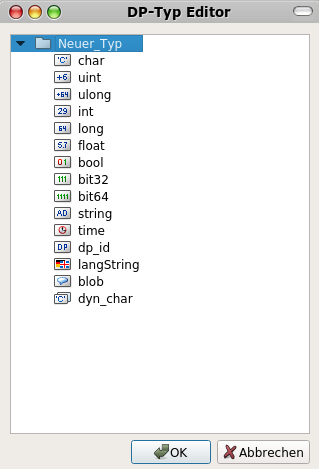
\includegraphics[width=0.40\textwidth]{dp_type}
	\caption{}
	\label{fig:dp_type}
\end{figure}

Die in Abbildung \ref{fig:dp_type}

\subsubsection{Datenpunkte}

\begin{figure}[h]
	\centering 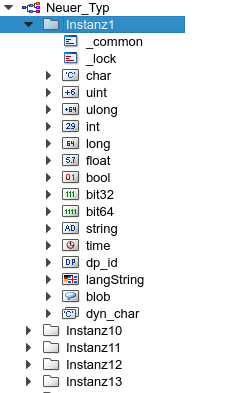
\includegraphics[width=0.35\textwidth]{dp_instances}
	\caption{}
	\label{fig:dp_instances}
\end{figure}

Die in Abbildung \ref{fig:dp_instances}

\subsubsection{Value Archive}

\subsection{Basis Agents und Konzept}

Je nach SCADA Produkt und Literatur werden die Teilnehmer eines solchen Systems unterschiedlich bezeichnet.
Während in dieser Arbeit der Begriff \textit{Agent} nach \cite{wooldridge_jennings_1995} Verwendung findet,
werden diese in WinCC OA als \textit{Manager} bezeichnet. Beide Begriffe folgen der vorher erläuterten Definition
für \textit{Agent}. Im kommenden Abschnitt werden die Basisprozesse eines WinCC OA Projekts beschrieben. 
Es wird dafür Bezug auf \cite{WinCCOA} genommen.

\subsubsection{Prozessmonitor}

Der Prozessmonitor startet und stoppt einzelne Prozesse eines WinCC OA Projektes und überwacht deren Status über zyklische
Anfragen. Im Fehlerfall versucht er den Prozess neu zu starten um somit ein stabiles gesamtsystem aufrecht zu erhalten.

\subsubsection{Event Manager}
Vermittelt anfragen etc.

\subsubsection{Data Manager}
Persistieren von Daten etc.

\subsubsection{Value Archive}
Historisches aufzeichnen von daten etc.

\subsubsection{Driver Manager}
Kommunizieren mit sps etc.

\subsubsection{Dist Manager}

\subsubsection{Redu Manager}

\subsubsection{API-Manager}

API

\subsection{C++-API}

WinCC OA stellt eine C++ Programmierschnittstelle zur Verfügung, mit der man eigene API Manager erstellen kann. 
Die Hauptfunktionen sind innerhalb zweier Singleton Klassen gekapselt.

\subsubsection{Manager Klasse}



\subsubsection{Resources Klasse}
\chapter{Google V8 Javascriptengine}
\label{cha:v8engine}

Während im letzten Kapitel auf die Konzepte und Funktionsweise von SCADA-Systemen eingegangen wurde, widmet sich dieses nun der Skriptsprache Javascript. 
Es wird gezeigt, wie diese Sprache technisch funktioniert. Als Javascriptengine bezeichnet man Programmkomponenten, die ECMA standardkonformen Quellcode ausführen können \cite{ecma}. 
Danach werden die drei bekanntesten Engines verglichen, um zu erläutern, warum die Google-V8-Engine für die Umsetzung gewählt wurde. 
Im letzten Abschnitt wird die Programmierschnittstelle dieser beschrieben. 

\section{Grundlagen}

Um zu verstehen, wie Javascript-Engines funktionieren, müssen die Grundlagen der Compilertheorie umrissen werden. Dazu wird
hier nun Bezug auf \cite{dragonBook} genommen. Als Compiler bezeichnet man ein Programm, das von Menschen lesbaren Quellcode
in binären Programmcode umwandelt, der von einem Computer ausgeführt werden kann. Im Folgenden wird die Theoretische
Funktionsweise eines solchen Programms beschrieben. 

, \cite{jsCore}, \cite{v8ByteCode}, \cite{jsSpiderMonkey}
Bevor das Umsetzungskonzept erläutert werden kann, muss die generelle Funktionsweise der Google V8 Javascriptengine
erörtert werden. Dazu wird in diesem Abschnitt Bezug auf \cite{v8embed} und \cite{v8mem} genommen.

\subsection{Contexts}

Ein Context ist eine Ausfuhrungsumgebung, die es ermöglicht, separaten, unabhängigen Javascript-Code in einer einzigen 
V8-Instanz (Isolate) auszufuhren. Da eine Isolate mehrere Context-Ausführungsumgebungen besitzen kann, muss jene, die zur 
Ausführung verwendet werden soll explizit angegeben werden. In dem Webbrowser \textit{Chromium} wird das Konzept der 
Contexts für je ein HTML Fenster oder \textit{iframe} verwendet.

\begin{figure}[h]
	\centering 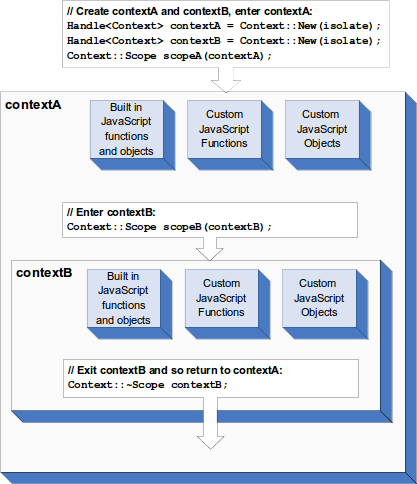
\includegraphics[width=0.7\textwidth]{contexts}
	\caption{In dieser Illustration wird die Unabhängigkeit der verschiedenen Contexts zueinander veranschaulicht.}
	\label{fig:contexts}
\end{figure}

In Abbildung \ref{fig:contexts} ist außerdem ersichtlich, dass mehrere Contexts auch verschachtelt aufgerufen 
werden können ohne sich gegenseitig zu beeinflussen.

\begin{figure}[h]
	\centering 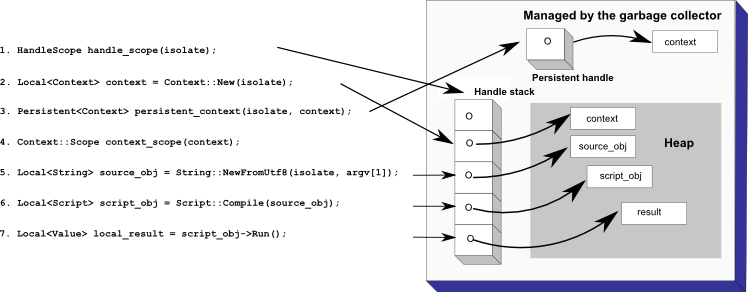
\includegraphics[width=1\textwidth]{handles}
	\caption{}
	\label{fig:handles}
\end{figure}

Jens

\section{Funktionsweise und Aufbau}

\subsection{Just-In-Time Compiler und Caches}

\subsection{Threadsicherheit mithilfe von Isolates}

1 Thread per Isolate, Locker Objekte

\subsection{Abgrenzen der Javascript-Ausführungsumgebungen mithilfe von Contexts}

Unabhängige ausführungsumgebung

\subsection{Speicherverwaltung}

Handles verwaltet über RAII geben Garbage collector auskunft über die validität von speicherzellen.

\subsection{Anpassen von Javascript-Ausführungsumgebungen über das Global Objekt}

\subsection{Das DebugInspector Protokoll}

\section{Vergleich mit anderen Javascript-Engines}
Vergleich vorallem mid Mozilla spidermonkey. Ev. auch performancetests.
\subsection{Mozilla SpiderMonkey}


\subsection{Apple JavaScriptCore}


\chapter{Anforderungen}
\label{cha:Anforderungen}

\section{Benutzerfreundlichkeit aus dem Gesichtspunkt der Systemintegratoren}

\section{Zu unterstützende Plattformen}

Vorgaben WinCC OA, zu 

\subsection{SUSE Linux Enterprise Server}

\subsection{Windows}

\section{Anwendungsfälle}

Use case diagramme + beschreibung etc.

\subsection{Remote-Fehleranalyse und Datenabfrage}

\subsection{Entwicklung kundenspezifischer Anforderungen}

\begin{figure}[h]
	\centering 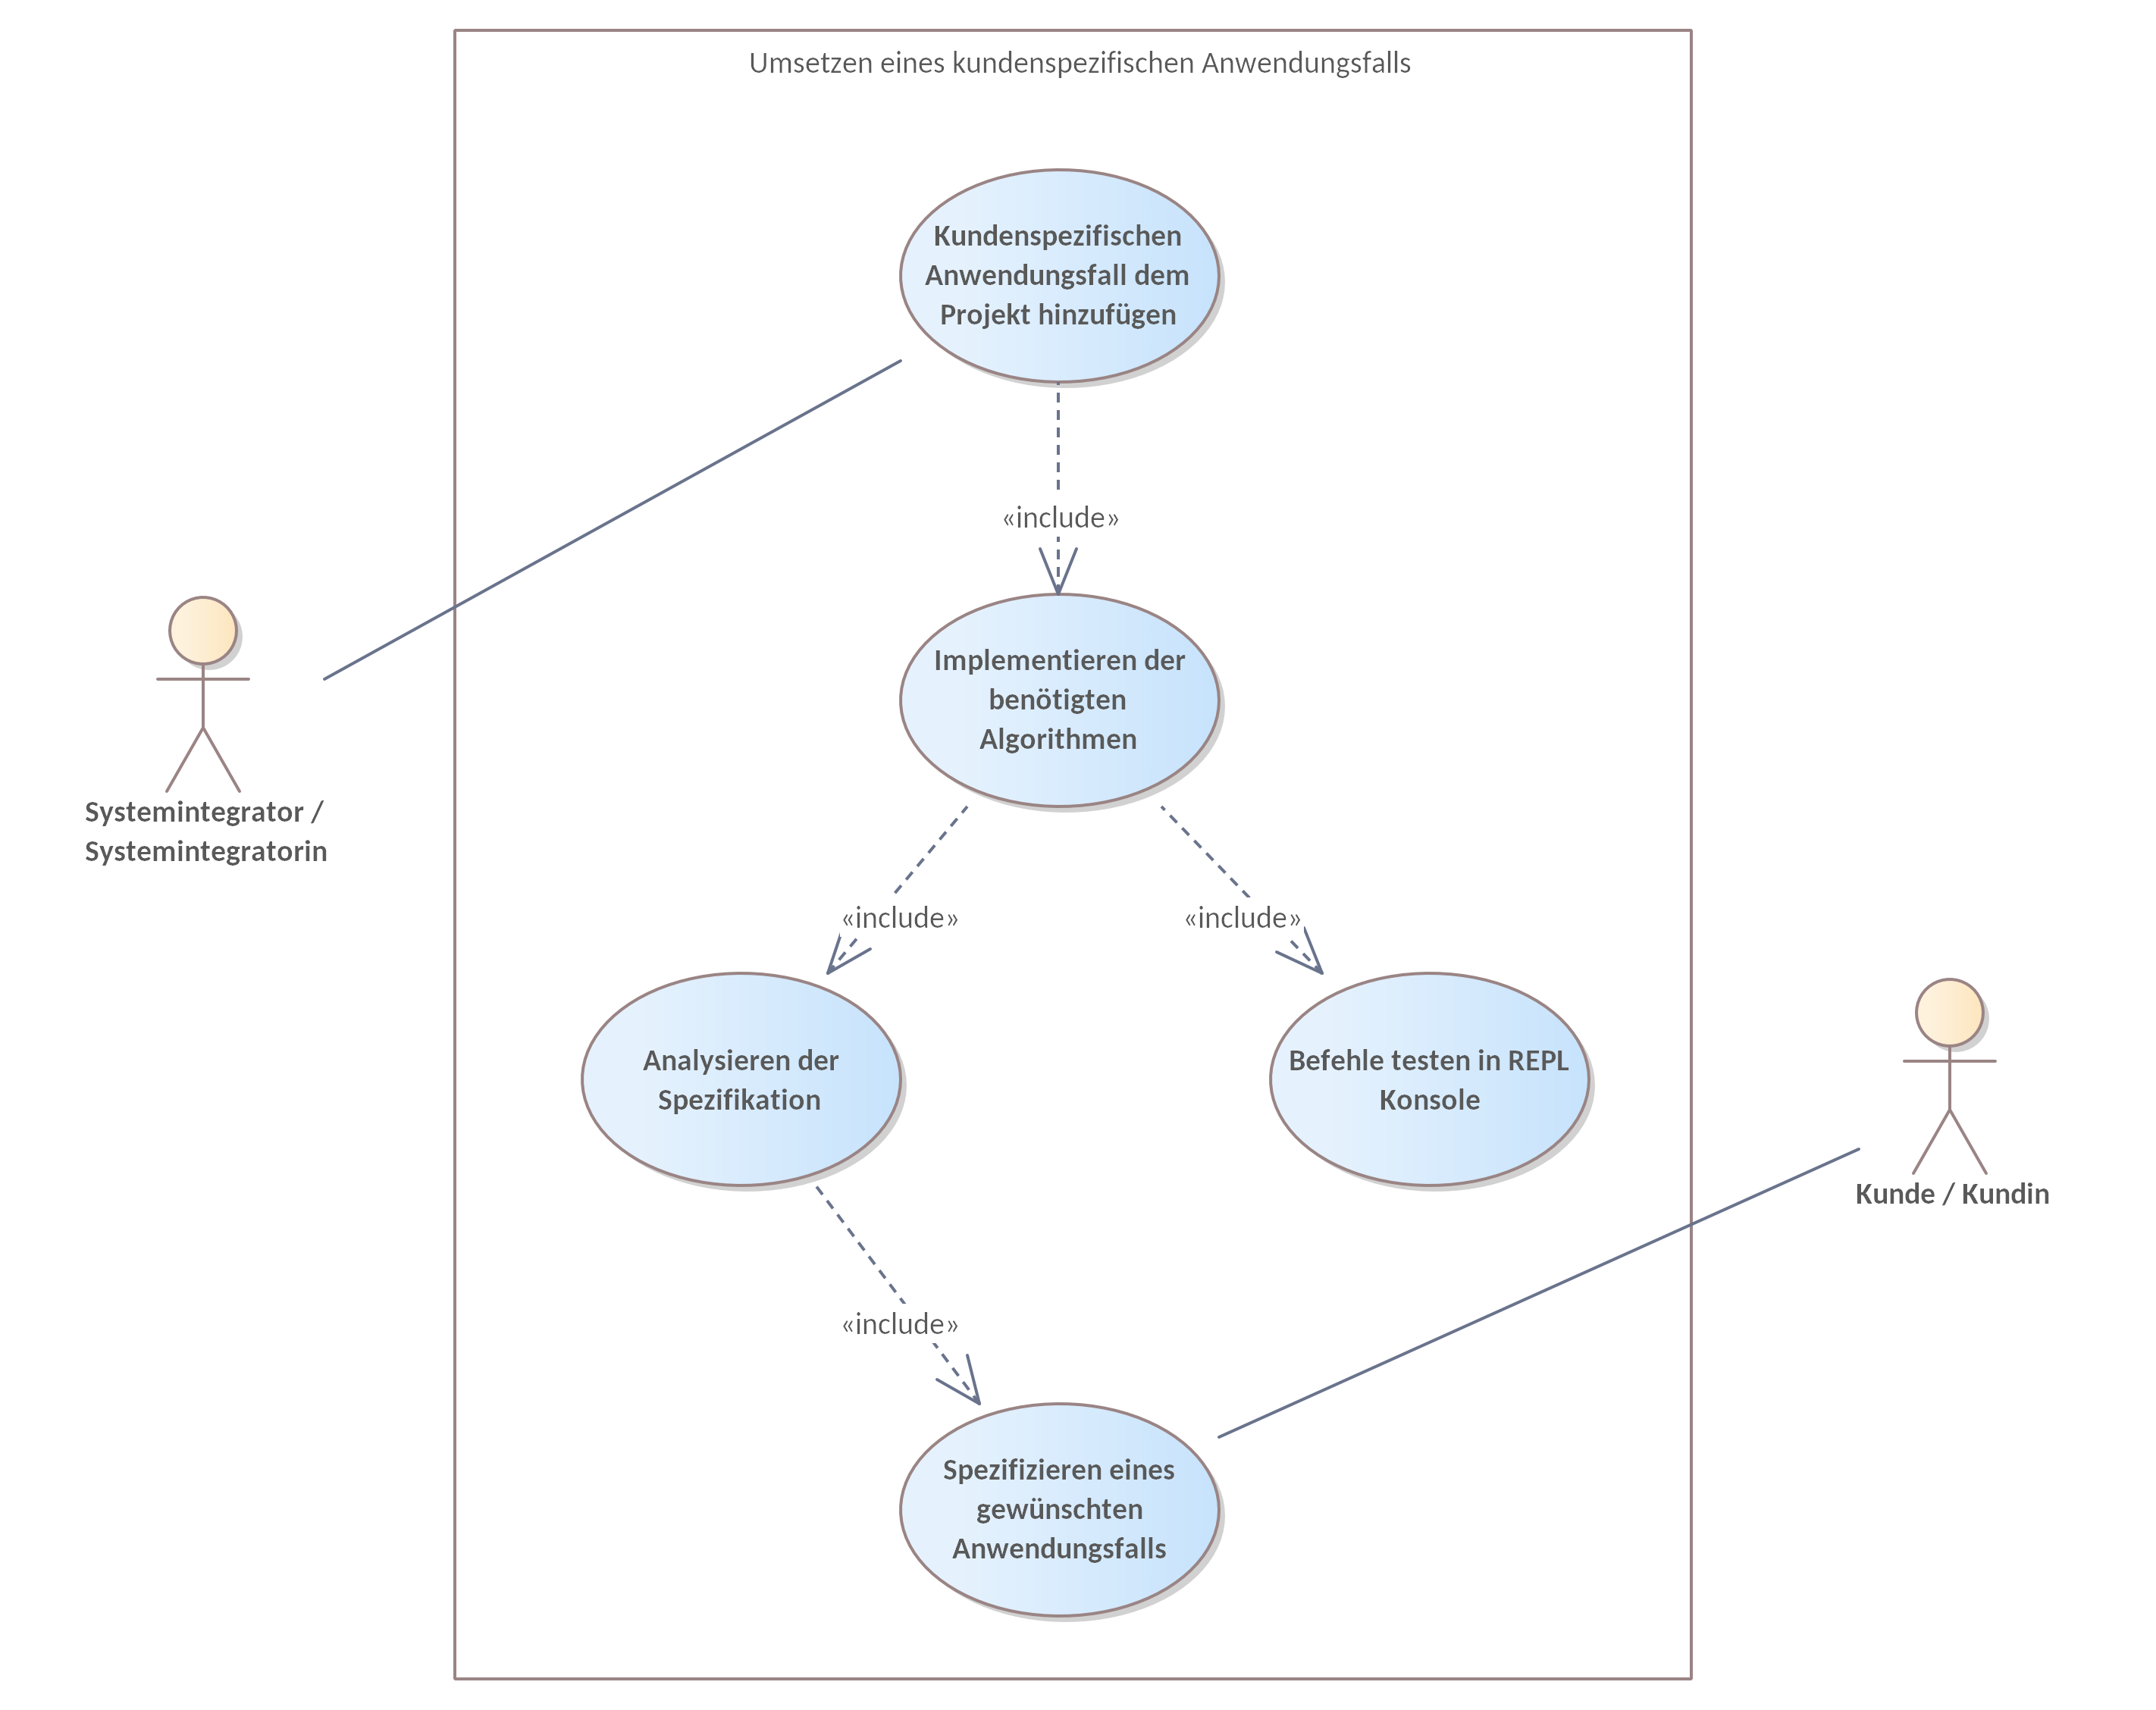
\includegraphics[width=1\textwidth]{UseCase_Implementation}
	\caption{a}
	\label{fig:UseCase_Implementation}
\end{figure}

In dem gezeigten Beispiel \ref{fig:UseCase_Implementation}

\subsection{Skriptgesützte Massenparametrierung}

\begin{figure}[h]
	\centering 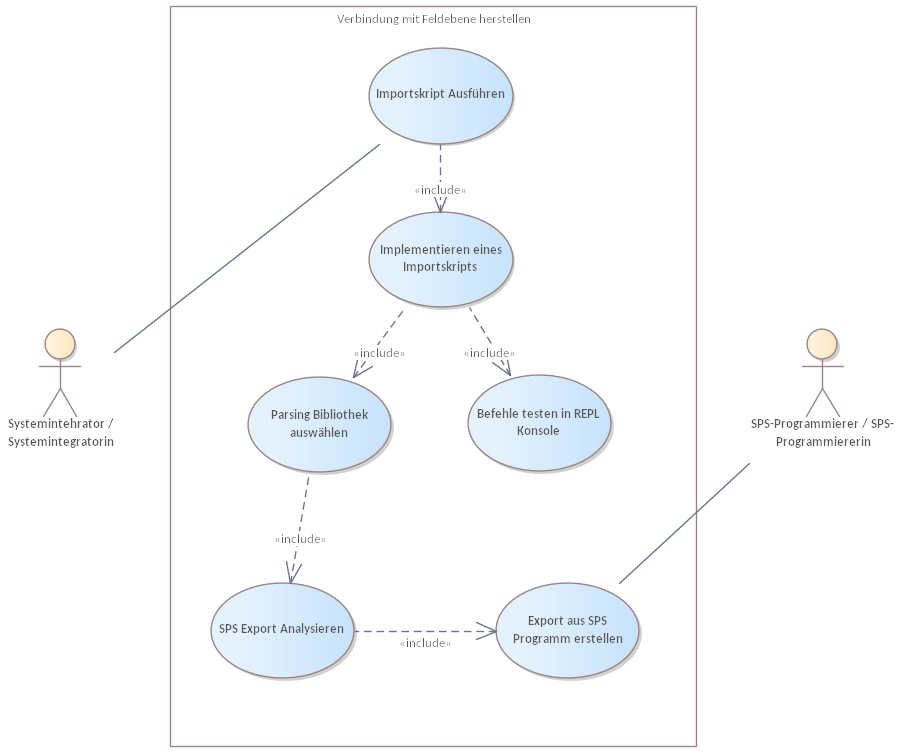
\includegraphics[width=1\textwidth]{UseCase_Import}
	\caption{a}
	\label{fig:UseCase_Import}
\end{figure}

In dem gezeigten Beispiel \ref{fig:UseCase_Import}

\section{Qualitätsanforderungen}

In diesen Abschnitt werden alle Punkte definiert, die die Qualität des Programmes aus Sicht der Systemintegratoren betreffen.

\subsection{Wiederverwendbare und dokumentierte C++-API}

\subsubsection{Verwendung als Templateengine}

Um statische HTML5 Dateien mit sich dynamisch ändernden Inhalten anzeigen zu können, kann man sogenanntes Templating verwenden. 
Hierbei wird eine Vorlage (HTML5 Datei) verarbeitet und bestimmte Platzhalter darin ähnlich wie bei einem Formular durch jeweils 
aktuelle oder speziell berechnete Inhalte ersetzt. Als Templateengine kann man hierbei ein serverseitiger Javascript-Interpreter, der Zugriff auf die Prozessdaten besitzt. 
Eine grafische Darstellung von Templating kann in folgendem Beispiel nachvollzogen werden \ref{fig:template_engine}: 

\begin{figure}[h]
	\centering 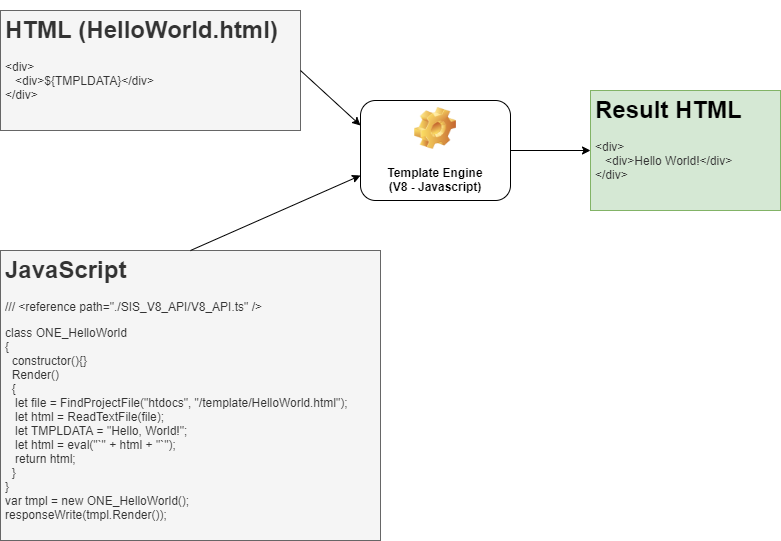
\includegraphics[width=1\textwidth]{template_engine}
	\caption{Funktionsweise Templating}
	\label{fig:template_engine}
\end{figure}

In dem gezeigten Beispiel \ref{fig:template_engine} kann man in HelloWorld.html \$\{TMPLDATA\} als Platzhalter erkennen. Dieser wird durch die 
Javascript Datei mit "Hello, World!" ersetzt. Links im Bild wird die resultierende HTML5 Datei gezeigt. 
Neue Agenten können sich dieser Mechanik bedienen, um individuelle Visualisierungen für die Clients zu erstellen.

\subsection{Digitales Handbuch für Integratoren als Nachschlagewerk}



\section{Wiederverwendbarkeit in spezifischeren C++-API-Agents}

\chapter{Konzept}
\label{cha:Konzept}

In diesem Kapitel wird ein Umsetzungskonzept für die im letzten Kapitel beschriebenen Anforderungen erarbeitet.


Umsetzung dll / lib / oder exe?

\section{Struktur der Programmbibliothek}
\subsection{Verwalten von Isolates und Contexts}
\subsection{Freilegen des DebugInspector Protokolls}
\subsection{Dynamische Parametrierung}

\section{Struktur des V8-API-Agenten}
\subsection{Parametrierung}

\section{Umsetzung}
\subsection{Zu verwendende Compiler}
\subsection{Benötigte Abhängigkeiten}
\subsection{Build Strategie}

\subsection{Compiler}

wahl der compiler auf linux und windows

\subsection{Handbuch Integratoren}

Typedoc / Doxygen.

\subsection{Linken externer Bibliotheken}

Im folgenden Abschnitt wird erklärt, wie ein Programm mit externen Bibliotheken umgehen kann. Die verschiedenen Möglichkeiten
werden dann abgewogen und in einem Fazit wird entschieden, welche Methode für den Prototyp verwendet wird.

\subsubsection{Statisches Linken}

Wird eine Bibliothek statisch gelinkt, dann werden die Funktionen dieser Bibliothek direkt in die ausführbare Datei kopiert.
Voraussetzung dafür ist, dass die gelinkte Bibliothek selbst statisch ist. Dies bedeutet, dass mindestens eine Objektdatei mithilfe des
Kommandozeilenprogrammes \textit{ar (archiver utility)} in ein Archiv umgewandelt wurde. \textit{Ar} fügt zu einem solchen Archiv eine Tabelle hinzu, in der vermerkt ist welche Symbole, wo im Archiv zu finden sind \cite{staticLinking}.

\subsubsection{Dynamisches Linken}

Beim dynamischen Linken werden die Funktionen einer dynamische Bibliothek in der ausführbaren Datei nur referenziert. Die dynamische
Bibliothek wird erst dann geladen, wenn das Programm gestartet wird. Ein wesentlicher Vorteil von dynamischen Bibliotheken gegenüber statischen
ist, dass der ausführbare Code für alle Prozesse, die diese Bibliothek benutzen nur einmal in den Speicher geladen wird \cite{dynLinking}.

\subsubsection{Fazit}

Da der Prototyp nur als einzelner Prozess laufen soll, ist durch die Verwendung von dynamischen Bibliotheken kein wirklicher Vorteil gegeben.
Es macht daher mehr Sinn alle externen Bibliotheken statisch in die ausführbare Datei zu linken, da man somit von externen Bibliotheken
unabhängig bleibt.

\chapter{Projektumsetzung}
\label{cha:Projektumsetzung}

In diesem Kapitel wird die Implementierung des SCADA-Agenten anhand des im letzten Kapitel aufgezeigten Konzeptes erläutert.

\section{Übersetzten des Google V8 C++ Quellcodes}

Dieser Abschnitt beschreibt wie die Google V8 Quellcode in eine statische Bibliothek übersetzt werden kann.

\subsection{Linux}

Aufgrund der Compilervorgaben von WinCC OA gestaltet sich die Übersetzung des Quellcodes auf Linux schwierig. 
Das Google V8 Buildsystem ist auf Debian-Basierende Distributionen ausgelegt, das bedeutet die Engine kann auf dem Zielsystem
SUSE Linux Enterprise 12.5 nicht übersetzt werden. Ein alternativsystem mit der passenden Compilerversion stellt Ubuntu 18.04
zur Verfügung.

\begin{program}[h]
\caption{Installation von GCC-4.8.5 auf Ubuntu 18.04}
\label{src:inst_gcc}
\begin{GenericCode}
$ sudo apt update
$ sudo apt upgrade
$ sudo apt install git libglib2.0-dev python g++-4.8 gcc-4.8
$ sudo update-alternatives --install /usr/bin/gcc gcc /usr/bin/gcc-4.8 10
$ sudo update-alternatives --install /usr/bin/g++ g++ /usr/bin/g++-4.8 10
\end{GenericCode}
\end{program}

In dem Beispiel \ref{src:inst_gcc} ist gezeigt wie man auf einem Ubutu 18.04 System den benötigten Compiler nachinstallieren und als
Standardoption zum Übersetzten von Quellcode konfigurieren kann. Hat man diese Schritte durchgeführt, kann man die Google V8-Engine mit dem in Anhang 
\ref{app:v8build} gezeigten Skript kompilieren. Dabei werden zuerst automatisch der Quellcode und alle benötigten Dateien aus dem Google-Versionskontrollsystem 
bezogen. Als Nächstes wird eine Buildkonfiguration erzeugt. In dieser wird das Buildsystem angewiesen eine statische
Bibliothek zu generieren. Danach erfolgt eine Nachbearbeitung der generierten Dateien, weil die Standardkonfiguration einen neueren Compiler
voraussetzt. Hierbei wird die \textit{-std=gnu++14} Anweisung durch \textit{-std=gnu++11} ersetzt. Letztendlich wird der Buildprozess 
gestartet. Die fertigen Kompilate sind unter \textit{v8} und die Headerdateien unter \textit{include} zu finden und können auf einem SUSE Linux Enterprise 12.5
System verwendet werden. 

\subsection{Windows}

Auf Windows gestaltet sich dieser Prozess deutlich einfacher. Hier ist es zunächst nötig, Visual Studio 2015 zu installiert. Dadurch wird das \textit{Visual Studio Toolset} v140
zur Verfügung gestellt. Im nächsten Schritt muss man das in \ref{app:v8build} gezeigte Powershell-Skript für Windows mit folgendem Kommandozeilenparameter ausführen: 

\begin{GenericCode}[numbers=none]
$ powershell.exe -noprofile -executionpolicy bypass -file .\build_windows.ps1
\end{GenericCode}

Dadurch wird ähnlich wie unter Linux der Quellcode und weitere Dateien aus dem Google-Versionskontrollsystem bezogen, die Konfigurationsdateien erzeugt
und der Kompilevorgang angestoßen. Die übersetzten Bibliotheksdateien und die dazugehörigen Headerdateien befinden sich danach unter \textit{v8} und \textit{include}.

\section{Implementierung der Programmbibliothek}

Nun, da erklärt wurde, wie man ein Kompilat der Google V8 Engine als statische Bibliothek erhält, kann die auf die Implementierung der 
Programmkomponente eingegangen werden. Hierbei werden die einzelnen Klassen anhand deren UML-Repräsentation (\textit{Unified Modeling Language}) 
beschrieben. Das gesamte UML-Diagramm mit allen Relationen kann in Anhang \ref{app:classdiag} eingesehen werden.

\subsection{Implementierung der Singleton Klasse}

\begin{figure}[h]
	\centering 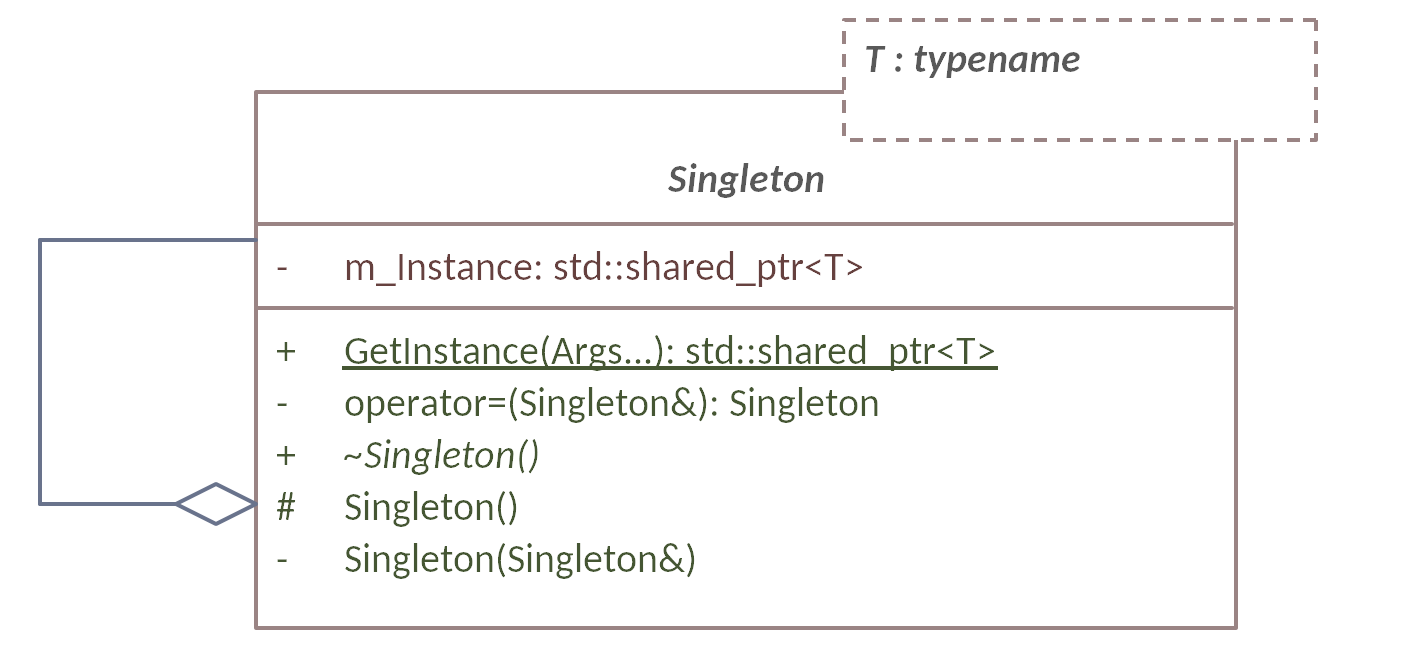
\includegraphics[width=0.63\textwidth]{singleton}
	\caption{Singleton Template-Klasse.}
	\label{fig:singleton}
\end{figure}

Diese in \ref{fig:singleton} gezeigte Template-Klasse implementiert eine wiederverwendbare Umsetzung des Singleton-Entwurfsmusters \cite{Singleton}. Ableitende Klassen erhalten indem sie
sich selbst als Template-Parameter übergeben eine \textit{GetInstance()} Funktion, die die einzige Instanz als \textit{Shared-Pointer} zurückgibt. 
Dadurch ist ein korrektes Freigeben des Speichers am Ende der Programmausführung gewährleistet. Ableitende Klassen müssen zusätzlich deren 
Konstruktor als \textit{protected} deklarieren und die Singleton klasse als \textit{friend} hinzufügen. Die \textit{GetInstance()} Methode nimmt
jene Parameter entgegen, die eine ableitende Klasse zur Konstruktion benötigt.

\subsection{Implementierung der libV8 Klasse}

\begin{figure}[h]
	\centering 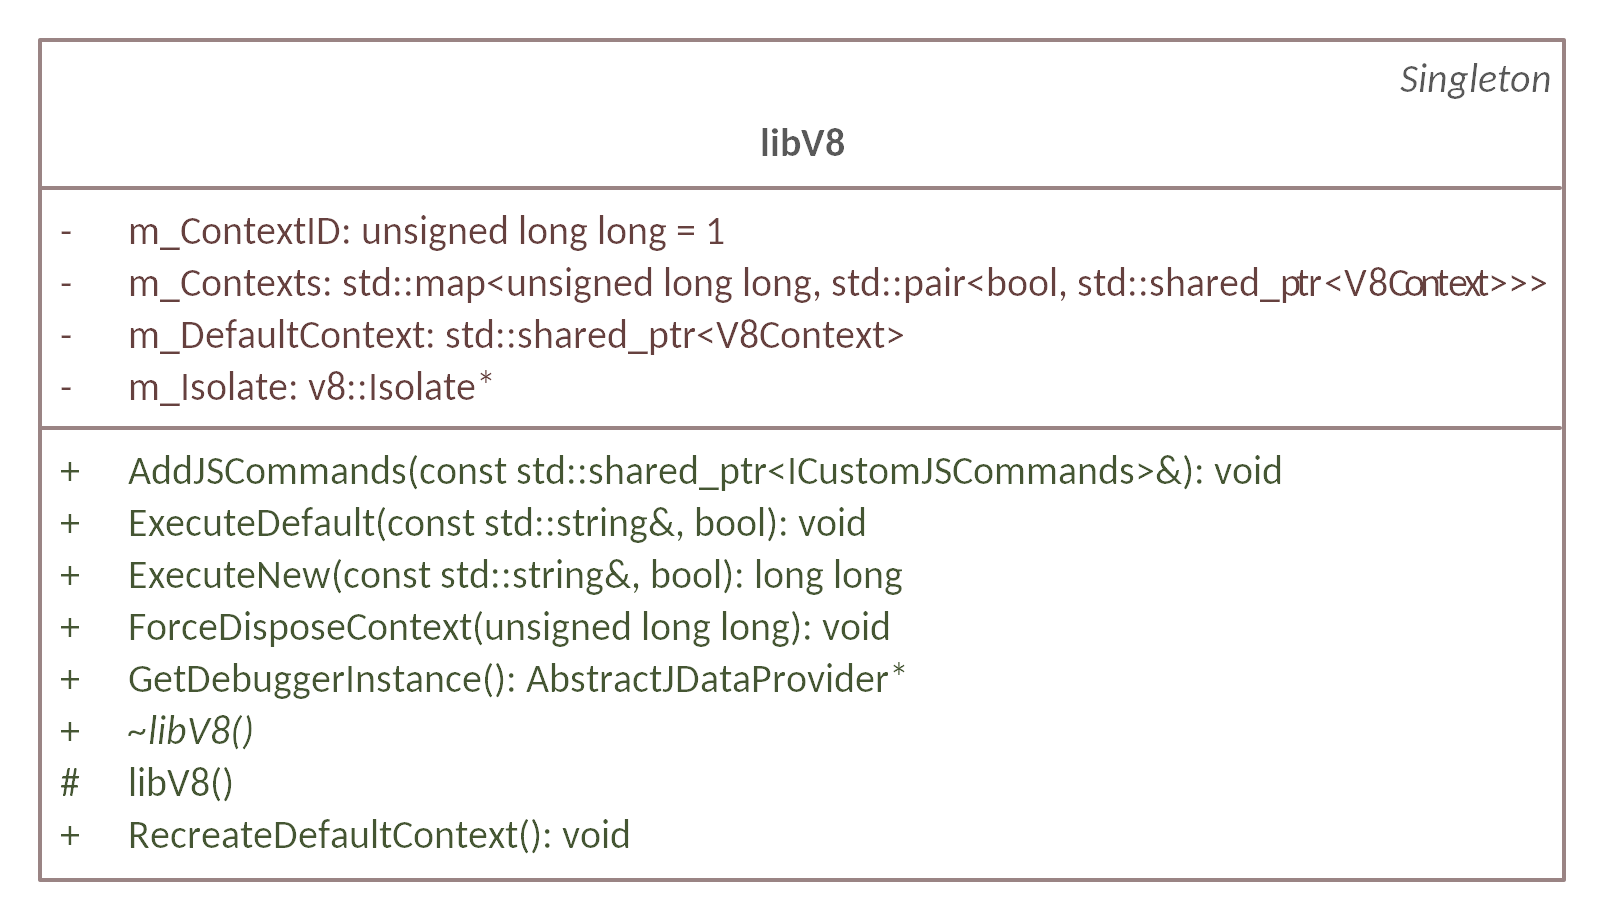
\includegraphics[width=0.63\textwidth]{libv8}
	\caption{Klassendiagramm der imlementierten Programmkomponente.}
	\label{fig:libv8}
\end{figure}

Abbildung \ref{fig:libv8} zeigt die Hauptkomponente der Bibliothek. Diese Klasse verwaltet das \textit{Isolate} Objekt der Google V8-Engine und alle
Ausführungsumgebungen. Über die Funktionen \textit{ExecuteDefault()} und \textit{ExecuteNew} ist es möglich Javascript-Dateien auszuführen. Beide akzeptieren
als ersten Parameter einen Pfad zu einer Skriptdatei und als zweiten einen booleschen wert der Angibt ob der Ausführungskontext am Ende des Skriptes zerstört 
werden soll oder nicht. 

\subsection{Implementierung der V8Context Klasse}


\begin{figure}[h]
	\centering 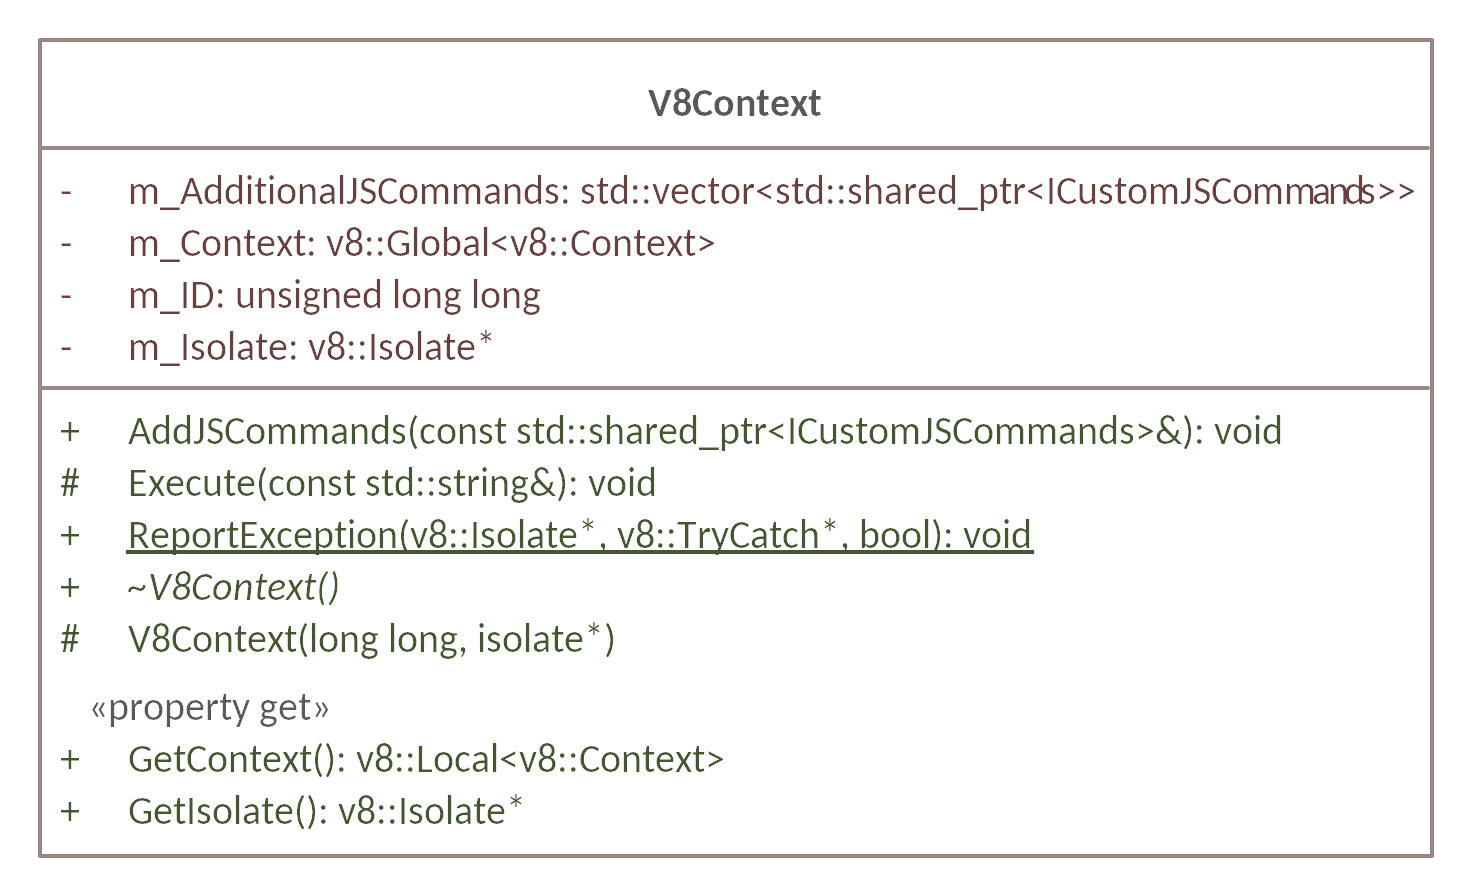
\includegraphics[width=0.63\textwidth]{v8context}
	\caption{Klassendiagramm der imlementierten Programmkomponente.}
	\label{fig:classdiag}
\end{figure}


\subsection{Implementierung der SIS\_InspectorClient Klasse}

\begin{figure}[h]
	\centering 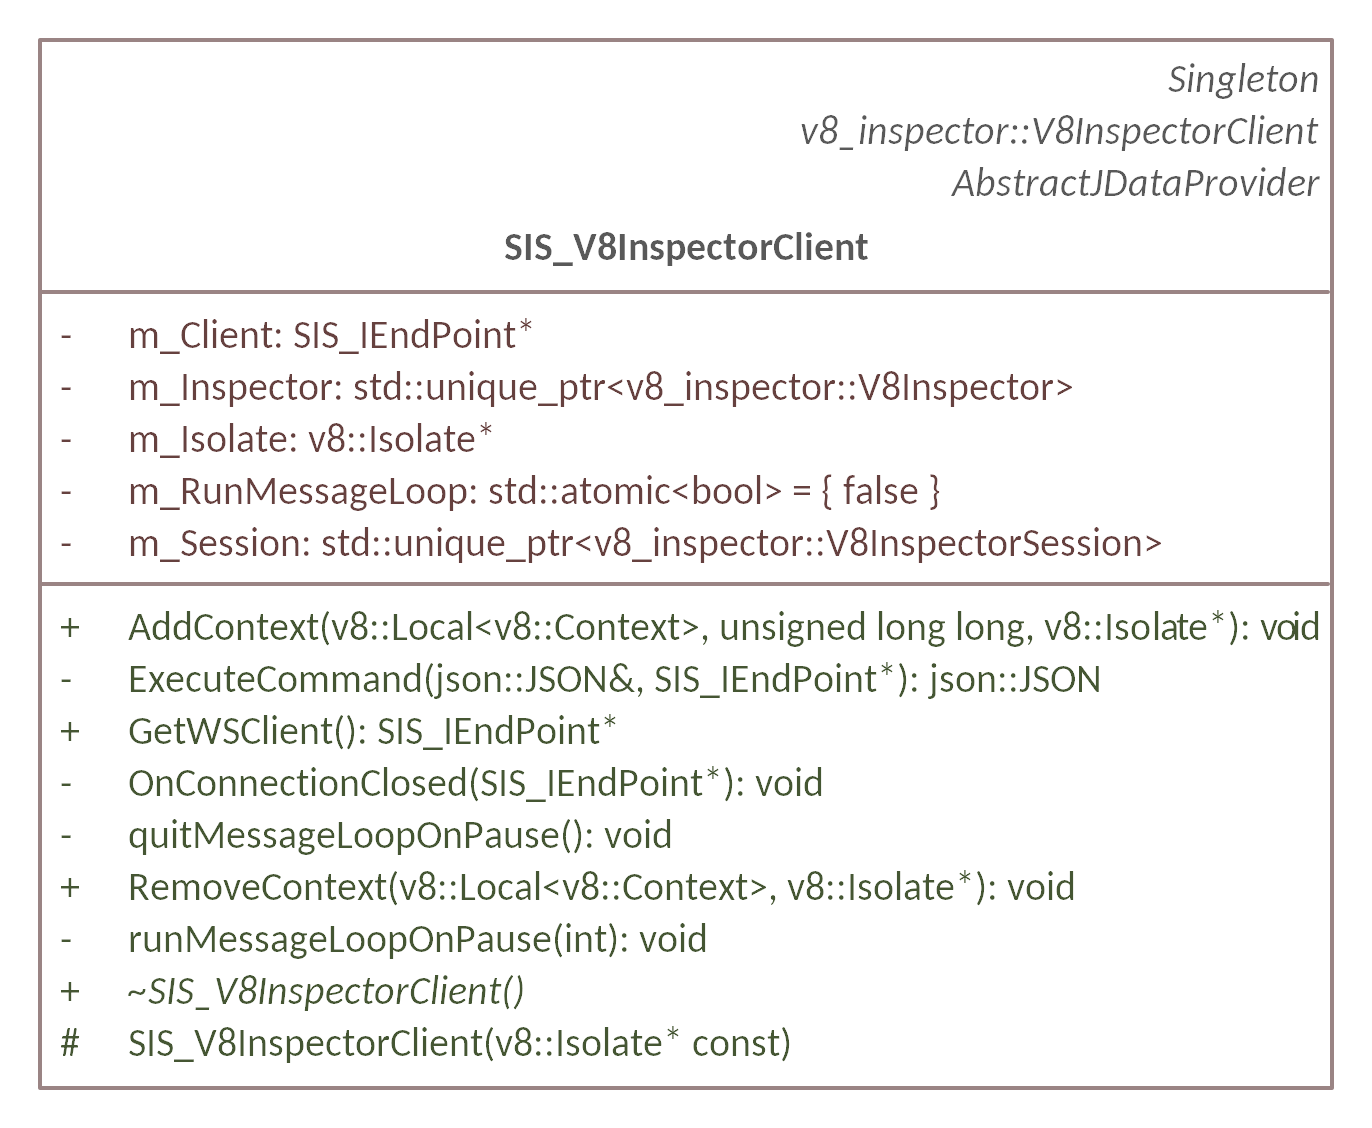
\includegraphics[width=0.63\textwidth]{inspectorclient}
	\caption{Klassendiagramm der imlementierten Programmkomponente.}
	\label{fig:classdiag}
\end{figure}

Die DebugInspector implementiert zusätzlich ein Interface für den in dem \textit{SiPlant} Produkt verwendten Websocket-Server.
Somit können

\subsection{Implementierung der SIS\_InspectorFrontend Klasse}

\begin{figure}[h]
	\centering 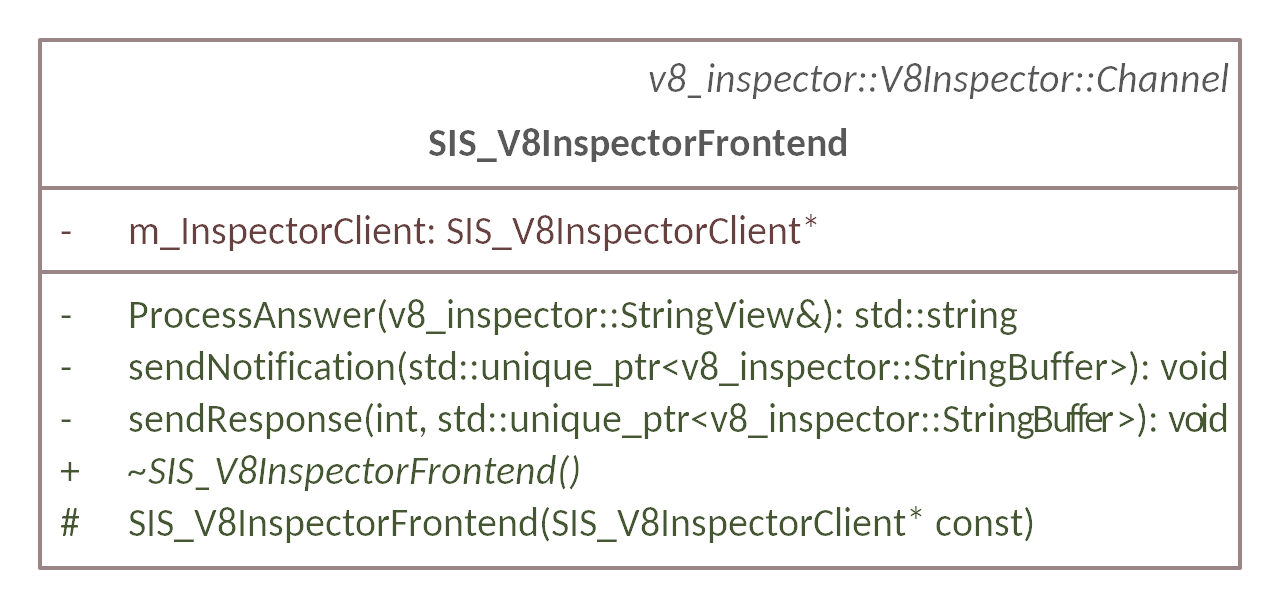
\includegraphics[width=0.63\textwidth]{inspectorfrontend}
	\caption{Klassendiagramm der imlementierten Programmkomponente.}
	\label{fig:classdiag}
\end{figure}

\subsection{Implementierung des ICustomJSCommands Interface}

\begin{figure}[h]
	\centering \includegraphics[width=0.63\textwidth]{icustomjscommands}
	\caption{Klassendiagramm der imlementierten Programmkomponente.}
	\label{fig:classdiag}
\end{figure}

\subsubsection{Konkretisierung DPJSCommands}

\begin{figure}[h]
	\centering 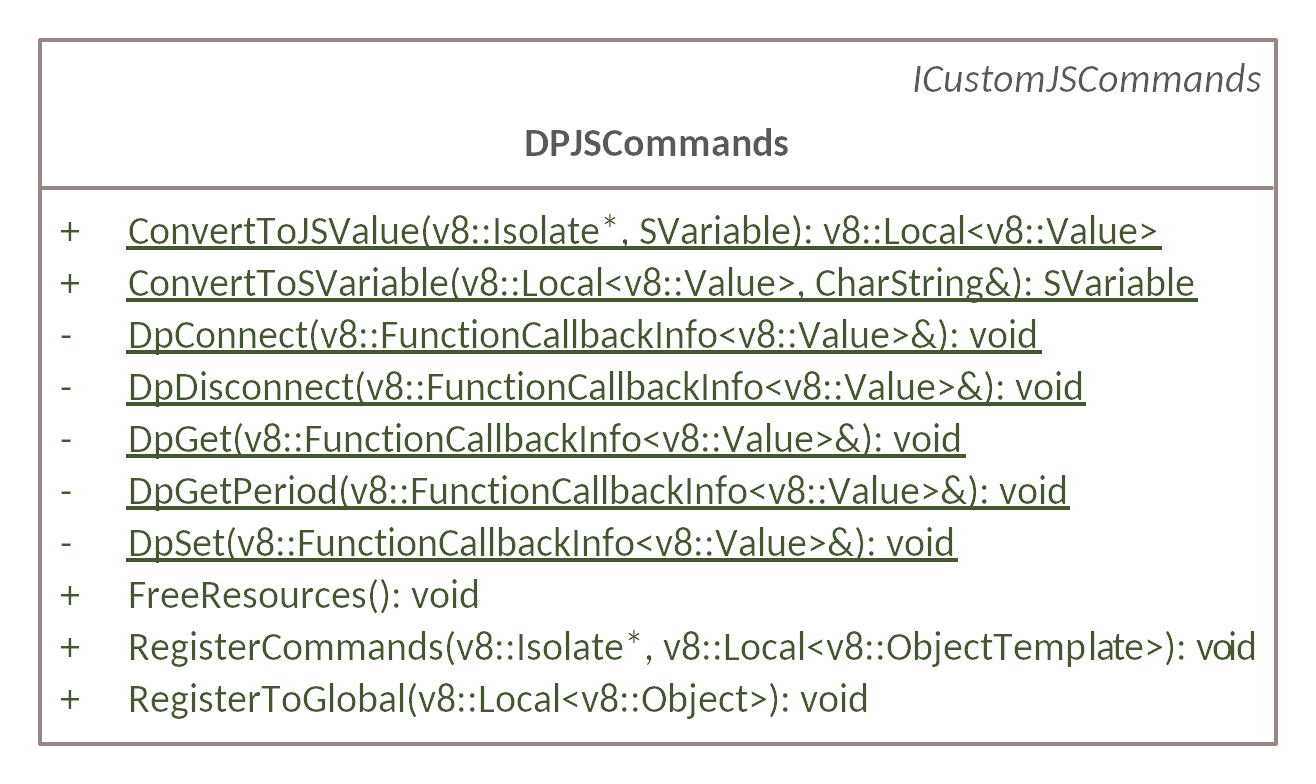
\includegraphics[width=0.63\textwidth]{dpjscommands}
	\caption{Klassendiagramm der imlementierten Programmkomponente.}
	\label{fig:classdiag}
\end{figure}

\subsubsection{Konkretisierung AlertJSCommands}

\begin{figure}[h]
	\centering 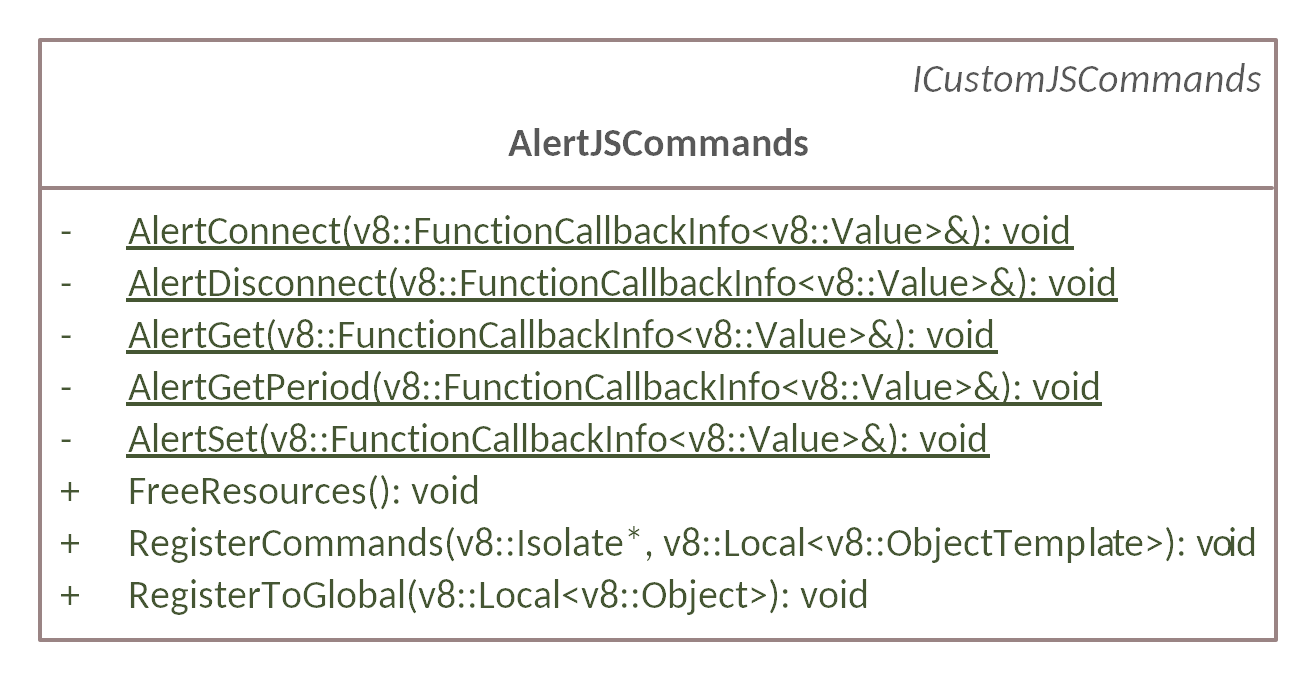
\includegraphics[width=0.63\textwidth]{alertjscommands}
	\caption{Klassendiagramm der imlementierten Programmkomponente.}
	\label{fig:classdiag}
\end{figure}


Dadurch ist es Umsetzungen diese Interfaces können 


\section{Implementierung des Agenten}

Der Agent verwendet die zuvor beschriebene Bibliothek, um Javascript-Dateien ausführen zu können. Die Datei ist über einen Kommandozeilenparameter 
übergebbar. In der Hauptfunktion ist am Anfang das Auslesen des Skriptpfades aus den übergebenen Parametern implementiert. Als Nächstes wird die Verbindung mit dem SCADA-System hergestellt. Darauf folgt das Starten des \textit{SiPlant} Websocket-Servers. Dieser erhält das von der \textit{GetDebuggerInstance()} Funktion zurückgegebenen Observer-Objekt. 
Dadurch ist ein Verbinden mit einer Browser-Entwicklerkonsole möglich. Danach wird vor der Hauptschleife mit dem wiederkehrenden 
\textit{dispatch()} Aufruf das übergebene Skript an die \textit{ExecuteDefault()} Funktion des texit{libV8()}-Singletons weitergereicht. 
Der boolesche Parameter ist hier auf 'false' gesetzt, da der Ausführungskontext nicht zerstört werden soll. Somit ist es möglich, 
eigene Algorithmen zu implementieren und eventorientiert Berechnungen in Javascript durchzuführen.

\chapter{Tests}
\label{cha:Tests}

\section{Ausgangssituation}
\label{sec:Ausgangssituation}

\section{Testsysteme}

\section{Testablauf}

\section{Testergebnisse}
\chapter{Zusammenfassung und Ausblick}
\label{cha:Zusammenfassung}

\section{Zusammenfassung}

\section{Ausblick}

\chapter{Danksagungen}
\label{cha:Danksagungen}

%%%----------------------------------------------------------
\appendix                                            % Anhang 
%%%----------------------------------------------------------

\chapter{Google V8 Javascriptengine Buildskripte}
\label{app:v8build}

\section{Linux}

\begin{GenericCode}
#!/bin/bash
# Author: Daniel Giritzer
# This script builds google V8 from source.
# To be used on Ubuntu 18.04
# to install and setup dependencies execute:
# sudo apt install git libglib2.0-dev python g++-4.8 gcc-4.8
# sudo update-alternatives --install /usr/bin/gcc gcc /usr/bin/gcc-4.8 10
# sudo update-alternatives --install /usr/bin/g++ g++ /usr/bin/g++-4.8 10
WORKDIR=$(pwd)
OUTDIR=$WORKDIR/v8
BUILDDIR=$WORKDIR/v8/out/v8
ARTEFACTDIR=$WORKDIR/lib/sles_x64-release
INCLUDEDIR=$WORKDIR/include
VERSIONTAG="6.2.414.5"

# clean
rm -rf $WORKDIR/.cipd
rm -rf $WORKDIR/.gclient
rm -rf $WORKDIR/.gclient_entries
rm -rf $WORKDIR/depot_tools
rm -rf $WORKDIR/v8

# get depot tools
git clone https://chromium.googlesource.com/chromium/tools/depot_tools.git

# add depot tools to path
OLDPATH=$PATH
export PATH=$PATH:$WORKDIR/depot_tools/

# get v8 source
fetch v8
cd $OUTDIR && git checkout $VERSIONTAG && gclient sync -j 4

# extract archive and create needed folders
mkdir -p $BUILDDIR
mkdir -p $ARTEFACTDIR

# set path to find build executables remove gn wrapper (not needed)
export PATH=$OLDPATH:$OUTDIR/third_party/depot_tools/:$OUTDIR/buildtools/linux64/
rm -rf $OUTDIR/third_party/depot_tools/gn

# build configuration
echo 'is_component_build = false' >> $BUILDDIR/args.gn
echo 'is_debug = false' >> $BUILDDIR/args.gn
echo 'target_cpu = "x64"' >> $BUILDDIR/args.gn
echo 'use_goma = false' >> $BUILDDIR/args.gn
echo 'goma_dir = "None"' >> $BUILDDIR/args.gn
echo 'v8_enable_backtrace = true' >> $BUILDDIR/args.gn
echo 'v8_enable_disassembler = true' >> $BUILDDIR/args.gn
echo 'v8_enable_object_print = true' >> $BUILDDIR/args.gn
echo 'v8_enable_verify_heap = true' >> $BUILDDIR/args.gn
echo 'v8_static_library = true' >> $BUILDDIR/args.gn
echo 'v8_use_external_startup_data = false' >> $BUILDDIR/args.gn
echo 'v8_use_snapshot = true' >> $BUILDDIR/args.gn
echo 'is_clang = false' >> $BUILDDIR/args.gn
echo 'use_sysroot = false' >> $BUILDDIR/args.gn

# generate build files
cd $OUTDIR && gn gen $BUILDDIR

# workaround to prevent build from failing with g++ 4.8.5, force use of C++11
find $BUILDDIR -type f -exec sed -i 's/-Werror//g' {} \;
find $BUILDDIR -type f -exec sed -i 's/-std=gnu++14/-std=gnu++11 -fPIC -D_GLIBCXX_USE_CXX11_ABI=0/g' {} \;

# start build with verbose output
ninja -v -j 4 -C $BUILDDIR d8

# copy resulting librariers
find $BUILDDIR -name *.a -exec cp {} $ARTEFACTDIR \;

# copy include directory
mkdir -p $INCLUDEDIR
cp -rf $OUTDIR/include/* $INCLUDEDIR
cp -rf $BUILDDIR/gen/include/inspector/ $INCLUDEDIR
\end{GenericCode}


\section{Windows}

\begin{GenericCode}
# Author: Daniel Giritzer
# This script builds google V8 from source.
# Execute from cmd via:
# powershell.exe -noprofile -executionpolicy bypass -file .\build_windows.ps1
$WORKDIR="$pwd"
$OUTDIR="$WORKDIR\v8"
$BUILDDIR="$WORKDIR\v8\out\v8"
$ARTEFACTDIR="$WORKDIR\lib\win-x64-release"
$INCLUDEDIR="$WORKDIR\include"
$VERSIONTAG="6.2.414.5"

# helper function for unpacking zip archives
Add-Type -AssemblyName System.IO.Compression.FileSystem
function Unzip
{
    param([string]$zipfile, [string]$outpath)
    [System.IO.Compression.ZipFile]::ExtractToDirectory($zipfile, $outpath)
}

# download depot_tools
$CLIENT = new-object System.Net.WebClient
$CLIENT.DownloadFile("https://storage.googleapis.com/chrome-infra/depot_tools.zip","depot_tools.zip")
Unzip "depot_tools.zip" "depot_tools"

# add depot tools to path
$env:DEPOT_TOOLS_WIN_TOOLCHAIN=0
$env:GYP_MSVS_VERSION=2015
$OLDPATH=$env:Path
$env:Path="$pwd\depot_tools;$OLDPATH"

# get files needed for windows build
gclient

# get v8 sourcecode
fetch v8
cd "$OUTDIR"
git checkout $VERSIONTAG
gclient sync

New-Item -ItemType directory -Path $BUILDDIR

# build configuration
Add-Content $BUILDDIR\args.gn 'is_component_build = false'
Add-Content $BUILDDIR\args.gn 'is_debug = false'
Add-Content $BUILDDIR\args.gn 'target_cpu = "x64"'
Add-Content $BUILDDIR\args.gn 'use_goma = false'
Add-Content $BUILDDIR\args.gn 'goma_dir = "None"'
Add-Content $BUILDDIR\args.gn 'v8_enable_backtrace = true'
Add-Content $BUILDDIR\args.gn 'v8_enable_disassembler = true'
Add-Content $BUILDDIR\args.gn 'v8_enable_object_print = true'
Add-Content $BUILDDIR\args.gn 'v8_enable_verify_heap = true'
Add-Content $BUILDDIR\args.gn 'v8_static_library = true'
Add-Content $BUILDDIR\args.gn 'v8_use_external_startup_data = false'
Add-Content $BUILDDIR\args.gn 'v8_use_snapshot = true'
Add-Content $BUILDDIR\args.gn 'is_clang = false'

# workaround to link using /MD
(Get-Content $OUTDIR\build\config\win\BUILD.gn).replace('/MT', '/MD') | Set-Content $OUTDIR\build\config\win\BUILD.gn

# generate build files
cd $OUTDIR
gn gen $BUILDDIR

# start build with verbose output
ninja -v -C $BUILDDIR d8

# copy artefacts
Get-ChildItem -Path "$BUILDDIR\*" -Include *.lib -Recurse | Copy-Item -Destination $ARTEFACTDIR

# copy include directory
Remove-Item -Recurse -Force $INCLUDEDIR
Copy-Item $OUTDIR\include -Recurse -Destination $INCLUDEDIR
Copy-Item $OUTDIR\gen\include -Recurse -Destination $INCLUDEDIR
\end{GenericCode}	% Technische Ergänzungen
\chapter{Inhalt der CD-ROM/DVD}
\label{app:cdrom}

Die CD-ROM/DVD beinhaltet den \textit{SiPlant} Quellcode in der Version 2.1 und diese Arbeit in \textit{\latex}-Form. 
\newline
\par
Der Inhalt dieser CD-ROM/DVD gliedert sich in folgende Verzeichnisse:
\begin{itemize}
\item \textbf{Thesis:} In dem Verzeichnis Thesis ist der \textit{\latex} Quellcode dieser Arbeit inklusive Versionskontrolle abgelegt. Das verwendete Versionskontrollsystem ist \textit{git} \cite{git}.
\item \textbf{corelib:} WinCC OA als Fremdfunktionsschnittstelle, ein Konzeptioneller Beweiß.
\item \textbf{SMF\_3P:} Hier sind folgende externen Komponenten mit Quellcode, Kompilat und Skripte zum Kompilieren abgelegt, die zum Übersetzten des im SMF\_Native Verzeichnis abgelegten Quellcodes benötigt werden: \textit{ACE} \cite{ACE}, \textit{boost} \cite{boost}, \textit{GTEngine}, \textit{mbedtls} \cite{mbedtls}, \textit{OpenSSL} \cite{OpenSSL}, \textit{SQLite} \cite{SQlite}, \textit{Google V8 Engine} \cite{v8engine} und \textit{WebsocketPP} \cite{websocketpp}.
\item \textbf{SMF\_Native:} Dieser Ordner beinhaltet den C++-Quellcode von \textit{SiPlant} in der Version 2.1.
\item \textbf{SMF\_Common:} Subprojekt mit Sammlungen von Sprachübersetzungsdateien, Farbdefinitionen und Datenpunktlisten (Version 2.1).
\item \textbf{SMF\_PlantVisu:} Erweiterndes Modul mit verschiedenen Auswertungen für die Anlagenvisualisierung (Version 2.1).
\item \textbf{SMF\_SmartScheduler:} In diesem Verzeichnis befindet sich die Schichtkalender-Erweiterung (Version 2.1).
\end{itemize}	% Inhalt der CD-ROM/DVD
\chapter{Ausgabe einer V8-Javascript-Exception}
\label{app:ReportException}

\lstinputlisting[
	label={src:proto2_reportexc},
	caption={Gibt den Inhalt eines V8-TryCatch Objektes aus.},
	numbers=left,
	language=C++,
	firstnumber=0,
	firstline=17,
	lastline=50]{prototype2/src/prototyp2.cpp}

	% Chronologische Liste der Änderungen
%\chapter{Klassendiagramm}
\label{app:classdiag}
Siehe nächste Seite.
\begin{figure}[h]
	\centering 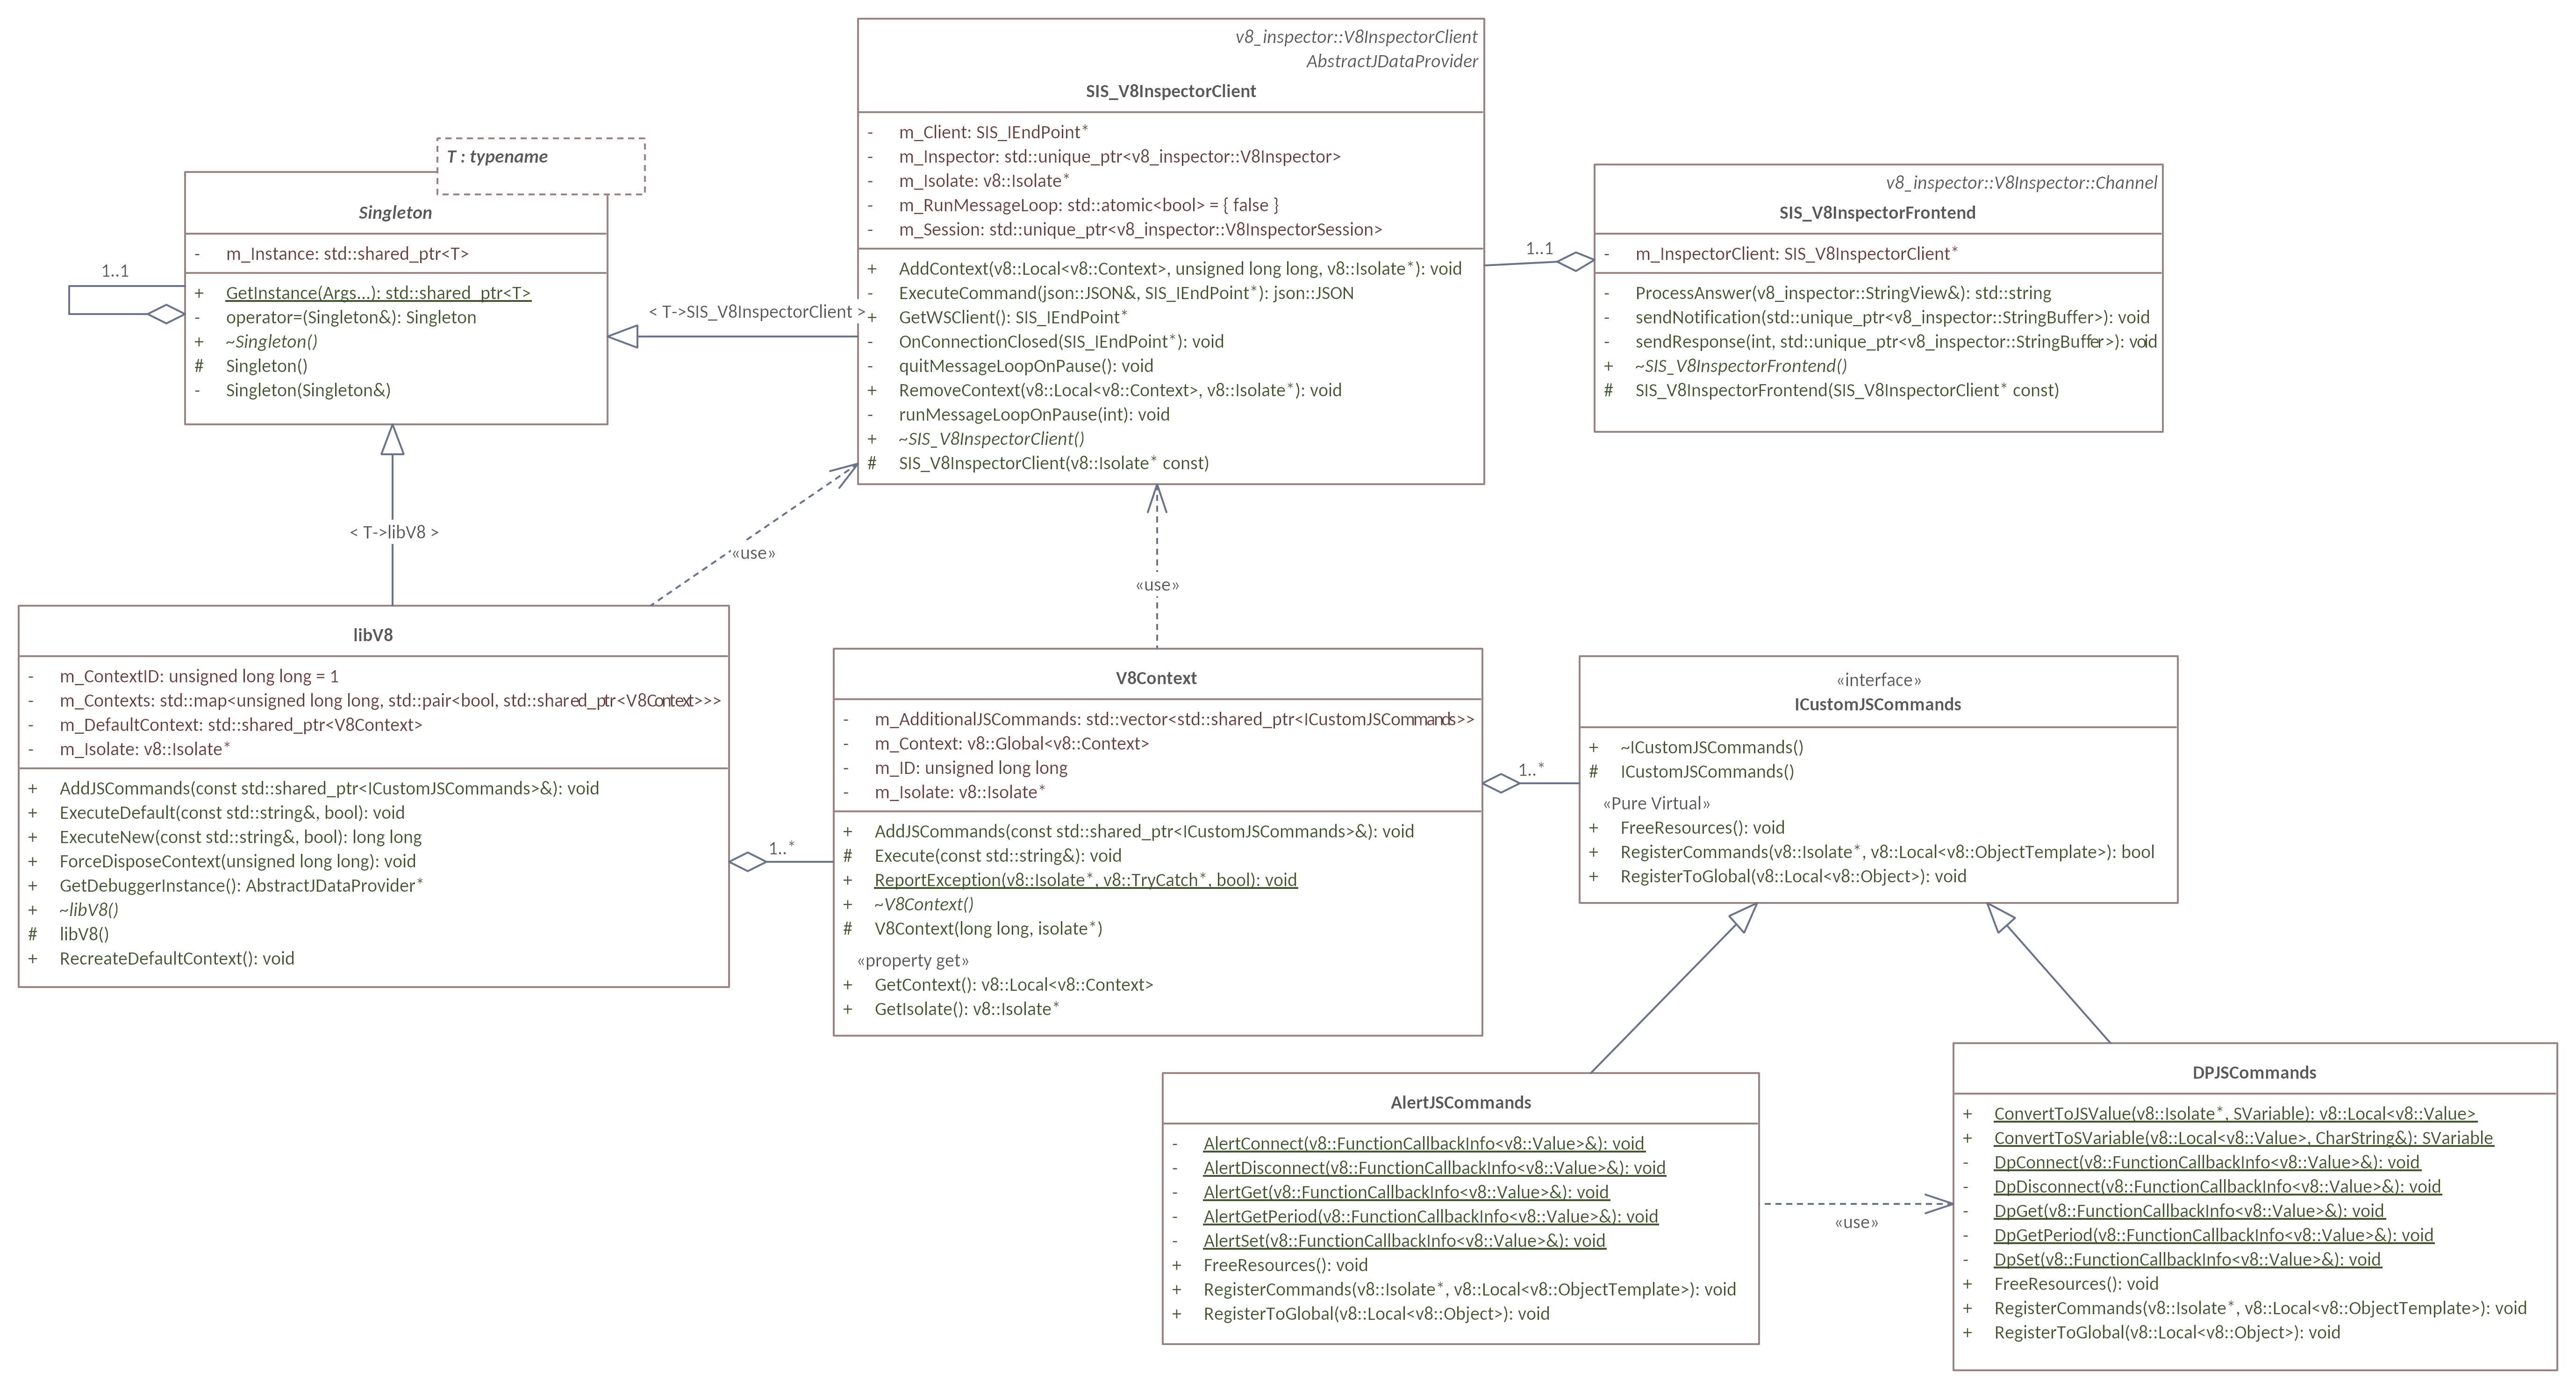
\includegraphics[width=1.73\textwidth,angle=90]{klassendiagramm_detailiert}
	\caption{Klassendiagramm der implementierten Programmkomponente.}
	\label{fig:classdiag}
\end{figure}	% Quelltext dieses Dokuments

\listoffigures
%%%----------------------------------------------------------
\MakeBibliography                        % Quellenverzeichnis
%%%----------------------------------------------------------

%%% Messbox zur Druckkontrolle ------------------------------
\chapter*{Messbox zur Druckkontrolle}



\begin{center}
{\Large --- Druckgröße kontrollieren! ---}

\bigskip

\calibrationbox{100}{50} % Angabe der Breite/Hoehe in mm

\bigskip

{\Large --- Diese Seite nach dem Druck entfernen! ---}

\end{center}



%%%----------------------------------------------------------
\end{document}
%%%----------------------------------------------------------